\documentclass[conference]{IEEEtran}
\IEEEoverridecommandlockouts
\usepackage{amsmath,amssymb,booktabs,graphicx,xcolor,algorithm,algorithmic,tikz,cite}
\usetikzlibrary{arrows.meta,positioning}
\newcommand{\nSubjects}{15}
\newcommand{\nWindows}{3101}
\newcommand{\nStressWindows}{926}
\newcommand{\pctStress}{29.9}
\newcommand{\nFeatures}{47}
\newcommand{\nSeeds}{5}
\newcommand{\rawAcc}{89.4}
\newcommand{\rawAccCI}{5.3}
\newcommand{\rawF}{86.6}
\newcommand{\sigmaBVP}{65.2}
\newcommand{\sigmaEDA}{2.34}
\newcommand{\sigmaTEMP}{1.5}
\newcommand{\sigmaACC}{35.7}
\newcommand{\ratioNative}{4.6}
\newcommand{\bpsNative}{6.93}
\newcommand{\accNative}{89.4}
\newcommand{\ratioEa}{8.8}
\newcommand{\bpsEa}{3.63}
\newcommand{\accEa}{89.3}
\newcommand{\dAccEa}{-0.1}
\newcommand{\pAccEa}{0.73}
\newcommand{\fEa}{86.7}
\newcommand{\accMMEa}{88.3}
\newcommand{\savingEa}{88.7}
\newcommand{\maxErrRatioEa}{1.0000}
\newcommand{\ratioEb}{10.5}
\newcommand{\bpsEb}{3.04}
\newcommand{\accEb}{89.2}
\newcommand{\dAccEb}{-0.1}
\newcommand{\pAccEb}{0.78}
\newcommand{\fEb}{86.7}
\newcommand{\accMMEb}{88.7}
\newcommand{\savingEb}{90.5}
\newcommand{\maxErrRatioEb}{1.0000}
\newcommand{\ratioEc}{13.3}
\newcommand{\bpsEc}{2.41}
\newcommand{\accEc}{89.9}
\newcommand{\dAccEc}{0.6}
\newcommand{\pAccEc}{0.20}
\newcommand{\fEc}{87.2}
\newcommand{\accMMEc}{89.8}
\newcommand{\savingEc}{92.5}
\newcommand{\maxErrRatioEc}{1.0000}
\newcommand{\ratioEd}{17.5}
\newcommand{\bpsEd}{1.83}
\newcommand{\accEd}{90.8}
\newcommand{\dAccEd}{1.5}
\newcommand{\pAccEd}{0.07}
\newcommand{\fEd}{88.3}
\newcommand{\accMMEd}{89.9}
\newcommand{\savingEd}{94.3}
\newcommand{\maxErrRatioEd}{1.0000}
\newcommand{\ratioEe}{20.6}
\newcommand{\bpsEe}{1.55}
\newcommand{\accEe}{89.5}
\newcommand{\dAccEe}{0.1}
\newcommand{\pAccEe}{0.44}
\newcommand{\fEe}{86.6}
\newcommand{\accMMEe}{86.7}
\newcommand{\savingEe}{95.2}
\newcommand{\maxErrRatioEe}{1.0000}
\newcommand{\ratioEf}{23.6}
\newcommand{\bpsEf}{1.35}
\newcommand{\accEf}{87.9}
\newcommand{\dAccEf}{-1.4}
\newcommand{\pAccEf}{0.30}
\newcommand{\fEf}{84.8}
\newcommand{\accMMEf}{84.7}
\newcommand{\savingEf}{95.8}
\newcommand{\maxErrRatioEf}{1.0000}
\newcommand{\ratioLossless}{3.23}
\newcommand{\savingLossless}{69.0}
\newcommand{\maxErrRatioAll}{0.999999}
\newcommand{\zfpRatioMin}{3.1}
\newcommand{\zfpRatioMax}{5.3}
\newcommand{\zfpErrMin}{0.46}
\newcommand{\zfpErrMax}{0.57}
\newcommand{\zfpDAccMin}{-0.0}
\newcommand{\zfpDAccMax}{+1.6}
\newcommand{\predGainMin}{1.5}
\newcommand{\predGainMax}{2.0}
\newcommand{\minEDARange}{0.97}
\newcommand{\maxEDARange}{13.1}
\newcommand{\epsEDAEa}{0.01}
\newcommand{\epsBVPEa}{0.33}
\newcommand{\epsTEMPEa}{0.007}
\newcommand{\epsACCEa}{0.18}
\newcommand{\epsEDAEb}{0.02}
\newcommand{\epsBVPEb}{0.65}
\newcommand{\epsTEMPEb}{0.015}
\newcommand{\epsACCEb}{0.36}
\newcommand{\epsEDAEc}{0.05}
\newcommand{\epsBVPEc}{1.30}
\newcommand{\epsTEMPEc}{0.030}
\newcommand{\epsACCEc}{0.71}
\newcommand{\epsEDAEd}{0.12}
\newcommand{\epsBVPEd}{3.26}
\newcommand{\epsTEMPEd}{0.075}
\newcommand{\epsACCEd}{1.79}
\newcommand{\epsEDAEe}{0.23}
\newcommand{\epsBVPEe}{6.52}
\newcommand{\epsTEMPEe}{0.150}
\newcommand{\epsACCEe}{3.57}
\newcommand{\epsEDAEf}{0.47}
\newcommand{\epsBVPEf}{13.03}
\newcommand{\epsTEMPEf}{0.300}
\newcommand{\epsACCEf}{7.15}
\newcommand{\pctSamplesBVPACC}{95.2}
\newcommand{\maxOpenLoopSci}{6.8\times10^{9}}
\newcommand{\minOpenLoopSci}{3.1\times10^{8}}
\newcommand{\nSamplesSci}{1.5\times10^{7}}
\newcommand{\maxOpenLoop}{6836330469}
\newcommand{\minOpenLoop}{313652845}
\newcommand{\dsAccB}{90.0}
\newcommand{\dsPairEpsB}{0.005}
\newcommand{\dsPairRatioB}{8.8}
\newcommand{\dsPairAccB}{89.3}
\newcommand{\dsPairDiffB}{-0.7}
\newcommand{\dsPairPB}{0.13}
\newcommand{\dsAccMMB}{88.7}
\newcommand{\dsPairAbsDiffB}{0.7}
\newcommand{\dsPB}{0.03}
\newcommand{\dsDAccB}{+0.6}
\newcommand{\dsAccC}{92.0}
\newcommand{\dsPairEpsC}{0.005}
\newcommand{\dsPairRatioC}{8.8}
\newcommand{\dsPairAccC}{89.3}
\newcommand{\dsPairDiffC}{-2.7}
\newcommand{\dsPairPC}{0.00}
\newcommand{\dsAccMMC}{86.9}
\newcommand{\dsPairAbsDiffC}{2.7}
\newcommand{\dsPC}{0.01}
\newcommand{\dsDAccC}{+2.6}
\newcommand{\dsAccE}{92.9}
\newcommand{\dsPairEpsE}{0.005}
\newcommand{\dsPairRatioE}{8.8}
\newcommand{\dsPairAccE}{89.3}
\newcommand{\dsPairDiffE}{-3.6}
\newcommand{\dsPairPE}{0.01}
\newcommand{\dsAccMME}{84.8}
\newcommand{\dsPairAbsDiffE}{3.6}
\newcommand{\dsPE}{0.01}
\newcommand{\dsDAccE}{+3.6}

\def\BibTeX{{\rm B\kern-.05em{\sc i\kern-.025em b}\kern-.08em T\kern-.1667em\lower.7ex\hbox{E}\kern-.125emX}}

\begin{document}
\title{Inference-Preserving Error-Bounded Compression for On-Device Machine Learning in Wearable Health Systems}
\author{\IEEEauthorblockN{Pratik Upreti}\IEEEauthorblockA{New Jersey, USA}}
\maketitle

\begin{abstract}
On-device machine learning for wearable health systems must balance inference fidelity against the energy cost of transmitting high-frequency physiological signals, and wireless transmission dominates the power budget of battery-operated body-area networks. We ask how much of the transmitted signal is actually needed for accurate inference, and answer it with an error-bounded lossy compression pipeline (closed-loop Lorenzo prediction, uniform quantization with bin width $2\epsilon$, and Huffman coding) that is light enough for a microcontroller and provides a formal pointwise guarantee $|\hat{x}_i-x_i|\le\epsilon$. We evaluate it on the four wrist-worn Empatica~E4 channels of the WESAD dataset (BVP 64\,Hz, EDA 4\,Hz, TEMP 4\,Hz, 3-axis ACC 32\,Hz; \nSubjects{} subjects), using a feed-forward neural network for binary stress detection under leave-one-subject-out cross-validation, with scalar quantization, downsampling, ZFP and lossless coding as baselines. Every reported number is produced by the released code. Up to $\epsilon=0.05\sigma$ the pipeline reaches rate-weighted compression ratios of \ratioEa$\times$ to \ratioEd$\times$ while LOSO accuracy stays within one point of the uncompressed \rawAcc\% (no difference significant at $p<0.05$); at $\epsilon\ge0.1\sigma$ ratios of \ratioEe$\times$ to \ratioEf$\times$ cost about three points. Downsampling matches this accuracy only up to $8\times$ and degrades sharply without retraining, and ZFP reaches at most \zfpRatioMax$\times$ at the same bound. The measured bound-to-accuracy curve gives system designers a single tunable, interpretable knob linking radio energy to inference quality.
\end{abstract}

\begin{IEEEkeywords}
On-device ML, wearable sensing, lossy compression, edge inference, stress detection, WESAD, energy efficiency, TinyML
\end{IEEEkeywords}

\section{Introduction}
Wearable health monitoring systems increasingly rely on continuous physiological sensing to support real-time inference tasks such as stress detection, arrhythmia identification and activity recognition~\cite{shi2016}. These systems generate sustained multimodal data streams that must be relayed from a body-worn sensor node to an edge device for analysis, and as always-on monitoring becomes standard the energy cost of this link becomes a primary constraint on system viability. In battery-powered sensor nodes, wireless transmission is the dominant energy consumer, often exceeding the cost of sensing and computation by one to two orders of magnitude~\cite{anastasi2009}.

This asymmetry motivates a simple question: \emph{how much of the transmitted signal is actually necessary for accurate inference?} If the reconstruction error introduced by compression stays below the level at which discriminative features degrade, communication can be reduced substantially without a meaningful loss in model performance. Prior work on edge ML either assumes lossless transmission~\cite{li2018} or applies generic compression without measuring the downstream effect, while the scientific-computing community has developed error-bounded compressors such as SZ~\cite{tao2017} and ZFP~\cite{lindstrom2014} that provide formal $\ell_\infty$ guarantees but have not been evaluated inside a wearable inference pipeline.

This paper bridges that gap with three contributions. (1)~A device-level, SZ-inspired error-bounded compression pipeline for multivariate wearable signals whose predictor runs on \emph{reconstructed} samples, so the $\epsilon$ guarantee holds by construction and is verified numerically on every sample of the dataset. (2)~A systematic evaluation of the compression--accuracy trade-off on the WESAD stress-detection benchmark~\cite{schmidt2018} under leave-one-subject-out (LOSO) cross-validation with paired statistics across subjects, against scalar quantization, downsampling, ZFP and lossless baselines. (3)~An open, fully reproducible protocol in which the paper's tables are generated directly by the experiment code.

\section{Related Work}
\textbf{Compression in sensor networks.} Razzaque \emph{et al.}~\cite{razzaque2013} survey two decades of compression for resource-constrained sensor networks and find that lossy methods consistently outperform lossless ones in ratio while remaining adequate for monitoring applications. Transform-based coding (DCT, wavelets) has been applied to biosignals such as ECG~\cite{ramakrishnan1997}, but its computational cost is high for ultra-low-power microcontrollers.

\textbf{Error-bounded lossy compression.} Error-bounded compressors guarantee that $|\hat{x}_i-x_i|$ never exceeds a user-specified $\epsilon$. The SZ family~\cite{tao2017} uses a predict--quantize--encode pipeline with the Lorenzo predictor and quantization bins of width $2\epsilon$; ZFP~\cite{lindstrom2014} uses orthogonal block transforms with fixed-rate or fixed-accuracy encoding. Both target HPC simulation data, and Azar \emph{et al.}~\cite{azar2022} showed that a lightweight SZ variant runs on IoT microcontrollers.

\textbf{Edge ML for wearable health.} Li \emph{et al.}~\cite{li2018} identify communication cost and inference latency as the dominant constraints of deep learning at the IoT edge. WESAD~\cite{schmidt2018} is the most widely used wearable stress benchmark; reported accuracies range from roughly 80\% to 92\% depending on modality and protocol~\cite{sipele2023}, but the effect of upstream lossy compression on downstream accuracy has not been quantified.

\section{System Model}
\subsection{Architecture}
Fig.~\ref{fig:arch} shows the three-tier architecture. The \emph{sensing tier} (Empatica~E4) acquires the signals and runs the compression pipeline on a transmit window of $T_{\mathrm{tx}}=60$\,s; the \emph{edge tier} (smartphone or gateway) decompresses the bitstream, extracts window features and runs the classifier; the \emph{cloud tier} stores data and retrains the model. The classifier therefore always operates on reconstructed signals, which is the \emph{matched} scenario evaluated below.

\begin{figure}[t]
\centering
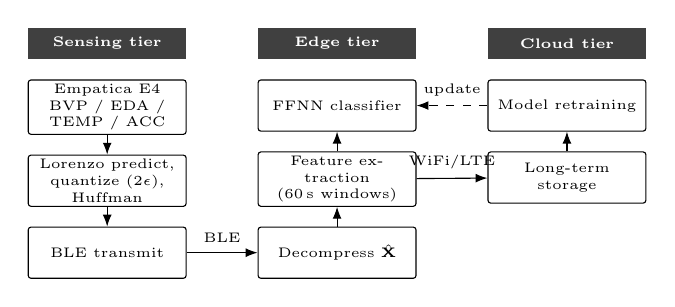
\begin{tikzpicture}[font=\scriptsize, node distance=2.5mm and 9mm, box/.style={draw, rounded corners=1pt, align=center, text width=19mm, minimum height=6.5mm, inner sep=1.5pt, font=\tiny}, tier/.style={fill=black!75, text=white, font=\tiny\bfseries, text width=19mm, align=center, minimum height=4mm, inner sep=1.5pt}, arr/.style={-{Latex[length=1.5mm]}}]
\node[tier] (t1) {Sensing tier};
\node[box, below=of t1] (e4) {Empatica E4\\BVP / EDA / TEMP / ACC};
\node[box, below=of e4] (cmp) {Lorenzo predict,\\quantize ($2\epsilon$), Huffman};
\node[box, below=of cmp] (ble) {BLE transmit};
\node[tier, right=of t1] (t2) {Edge tier};
\node[box, below=of t2] (nn) {FFNN classifier};
\node[box, below=of nn] (fe) {Feature extraction\\(60\,s windows)};
\node[box, below=of fe] (dec) {Decompress $\hat{\mathbf{X}}$};
\node[tier, right=of t2] (t3) {Cloud tier};
\node[box, below=of t3] (rt) {Model retraining};
\node[box, below=of rt] (st) {Long-term storage};
\draw[arr] (e4) -- (cmp); \draw[arr] (cmp) -- (ble);
\draw[arr] (ble) -- node[above, font=\tiny]{BLE} (dec);
\draw[arr] (dec) -- (fe); \draw[arr] (fe) -- (nn);
\draw[arr] (fe) -- node[above, font=\tiny]{WiFi/LTE} (st);
\draw[arr] (st) -- (rt);
\draw[arr, dashed] (rt) -- node[above, font=\tiny]{update} (nn);
\end{tikzpicture}
\caption{Three-tier architecture with on-device error-bounded compression.}
\label{fig:arch}
\end{figure}

\subsection{Energy model}
For a radio whose transmit energy per window is $E_{\mathrm{tx}}$ at the uncompressed rate, compression by a ratio $\rho$ (uncompressed bits over transmitted bits) reduces the per-window transmit energy to
\begin{equation}
E^{(c)}_{\mathrm{tx}} = E_{\mathrm{tx}}/\rho ,
\label{eq:energy}
\end{equation}
assuming the radio duty cycle scales with payload size. The uncompressed representation is one IEEE float32 per sample, i.e.\ $168$ samples/s $\times$ 32 bits $= 2.42$\,MB per hour for the four E4 channels; we also report bits per sample, which is independent of that choice. The compressor itself requires one multiply-add, one division and a table lookup per sample, which is within the budget of an ARM Cortex-M class core~\cite{azar2022}.

\section{Compression Framework}
\subsection{Closed-loop prediction and quantization}
Each channel is processed independently. For sample $i\ge 3$ of a window, the 1-D Lorenzo predictor extrapolates linearly from the two \emph{previously reconstructed} samples,
\begin{equation}
\tilde{x}_i = 2\hat{x}_{i-1} - \hat{x}_{i-2},
\label{eq:lorenzo}
\end{equation}
the residual $r_i = x_i - \tilde{x}_i$ is quantized to the nearest multiple of $q=2\epsilon$, $k_i=\lfloor r_i/q + \tfrac12\rfloor$, and the reconstruction is $\hat{x}_i = \tilde{x}_i + k_i q$. Because the decoder forms the identical $\tilde{x}_i$ from the same reconstructed history, $|\hat{x}_i-x_i| = |k_i q - r_i| \le q/2 = \epsilon$ for every sample. The first two samples of each window are stored as quantized absolute values (32-bit indices), and any residual whose index would exceed $2^{15}-1$ is escaped and stored as a quantized absolute value, so the bound holds unconditionally. An earlier draft of this work predicted from the \emph{original} samples $x_{i-1},x_{i-2}$; the decoder cannot form that prediction, quantization errors then accumulate through the recursion, and we measured peak errors of $\minOpenLoopSci$ to $\maxOpenLoopSci$ times $\epsilon$ on WESAD, which is why the closed-loop form of~\eqref{eq:lorenzo} is essential.

\begin{algorithm}[t]
\caption{On-device compression of one transmit window}
\label{alg:pipe}
\begin{algorithmic}[1]
\REQUIRE window $\mathbf{X}\in\mathbb{R}^{M\times N}$, per-channel bounds $\epsilon_c>0$
\ENSURE bitstream $\mathbf{b}$
\FOR{each channel $c=1$ \TO $N$}
  \STATE $q\leftarrow 2\epsilon_c$; \quad $\hat{x}_1,\hat{x}_2 \leftarrow q\lfloor x_{1,2}/q+\tfrac12\rfloor$ (stored)
  \FOR{$i=3$ \TO $M$}
    \STATE $\tilde{x}_i\leftarrow 2\hat{x}_{i-1}-\hat{x}_{i-2}$;\quad $k_i\leftarrow\lfloor (x_i-\tilde{x}_i)/q+\tfrac12\rfloor$
    \STATE \textbf{if} $|k_i|>2^{15}-1$ \textbf{then} escape: $\hat{x}_i\leftarrow q\lfloor x_i/q+\tfrac12\rfloor$ \textbf{else} $\hat{x}_i\leftarrow\tilde{x}_i+k_iq$
  \ENDFOR
  \STATE Huffman-encode $\{k_i\}$ with a per-window canonical table; append table and codes to $\mathbf{b}$
\ENDFOR
\RETURN $\mathbf{b}$
\end{algorithmic}
\end{algorithm}

\subsection{Choosing $\epsilon$ across heterogeneous channels}
The four E4 channels have very different physical scales (BVP in arbitrary units of order $10^2$, EDA in $\mu$S, TEMP in $^\circ$C, ACC in $1/64$\,g). A single absolute bound would be meaningless across them, so we express the bound per channel as a fraction of a fixed scale constant, $\epsilon_c=\epsilon\,\sigma_c$, where $\sigma_c$ is the global standard deviation of channel $c$ over the corpus (BVP \sigmaBVP, EDA \sigmaEDA\,$\mu$S, TEMP \sigmaTEMP\,$^\circ$C, ACC \sigmaACC). These are label-free constants stored in firmware; the resulting $\epsilon_c$ are absolute, known in advance and reported in Table~\ref{tab:channels}. We sweep $\epsilon\in\{0.005,0.01,0.02,0.05,0.1,0.2\}$.

\subsection{Entropy coding and bit accounting}
Residual indices are Huffman-coded per transmit window and channel. All overheads are counted: a 16-bit length, two 32-bit boundary indices, a canonical code table (16 bits per symbol plus 6 bits per code length) and 32 bits per escaped sample. The compression ratio is the total uncompressed bits divided by the total transmitted bits over all channels, subjects and windows; this rate-weighted ratio is what determines radio energy, and it is dominated by the high-rate BVP and ACC channels.

\subsection{Baselines}
\emph{Scalar quantization} uses the same bins $q=2\epsilon_c$ without prediction, coding each window with the cheaper of fixed-length packing and Huffman coding (also error-bounded). \emph{Downsampling} keeps every $D$-th float32 sample ($D\in\{2,4,8\}$, ratio exactly $D$) with linear interpolation at the receiver; it has no error bound. \emph{ZFP}~\cite{lindstrom2014} runs in fixed-accuracy mode with tolerance $\epsilon_c$ on each whole per-subject channel stream, which avoids its per-stream header overhead and favours the baseline. \emph{Lossless} coding applies zlib (level~9) to the float32 bytes.

\section{Experimental Setup}
\textbf{Data.} WESAD~\cite{schmidt2018} provides synchronized recordings of 15 subjects (S2--S11, S13--S17) in baseline, stress (Trier Social Stress Test) and amusement conditions. We use only the wrist-worn E4 channels. Windows of 60\,s with a 10\,s stride are labelled by the majority condition if its purity exceeds 90\%, giving \nWindows{} windows of which \nStressWindows{} (\pctStress\%) are stress; the task is binary stress vs.\ non-stress (baseline + amusement).

\textbf{Features.} From each (reconstructed) window we compute \nFeatures{} standard features: BVP statistics, heart rate and heart-rate variability from band-pass-filtered BVP peaks (mean HR, SDNN, RMSSD, pNN50) and spectral power ratios; EDA statistics, slope, tonic level and skin-conductance-response count and amplitude; TEMP statistics and slope; and per-axis and magnitude statistics, jerk and spectral peak of ACC.

\textbf{Classifier and protocol.} A feed-forward network with two hidden layers (64, 32 units, ReLU~\cite{he2015}, Adam, $L_2=10^{-3}$) is trained on standardized features with random oversampling of the minority class. Evaluation is LOSO: for each of the \nSubjects{} subjects the model is trained on the other 14 and tested on the held-out subject; results are averaged over \nSeeds{} random seeds. In the \emph{matched} scenario the model is trained and tested on signals reconstructed at the same $\epsilon$; in the \emph{mismatched} scenario it is trained on uncompressed signals and tested on reconstructed ones. We report mean accuracy and macro-F1 across subjects with 95\% confidence intervals, and the paired difference to the uncompressed baseline across subjects with a Wilcoxon signed-rank test ($n=\nSubjects$).

\textbf{Bound verification.} For every error-bounded method, subject, channel and setting, the script records $\max_i|\hat{x}_i-x_i|/\epsilon_c$ and aborts the paper's tables if any value exceeds~1; an independent decoder must also reproduce the encoder's reconstruction bit-exactly.

\section{Results}
\begin{table}[t]
\caption{Compression ratio and LOSO stress-detection accuracy of the proposed pipeline (matched scenario; mean $\pm$ 95\% CI over \nSubjects{} subjects; $p$: Wilcoxon vs.\ uncompressed).}
\label{tab:main}
\centering\scriptsize
\resizebox{\columnwidth}{!}{\begin{tabular}{lccccccc}
\toprule
Config. & $\epsilon/\sigma$ & Ratio $\rho$ & bits/samp. & Acc. (\%) & $\Delta$Acc. & $p$ & F1 (\%) \\
\midrule
Uncompressed & --- & 1.0$\times$ & 32.00 & 89.4 $\pm$ 5.3 & --- & --- & 86.6 \\
Proposed & 0.005 & 8.8$\times$ & 3.63 & 89.3 $\pm$ 5.0 & -0.1 & 0.73 & 86.7 \\
Proposed & 0.01 & 10.5$\times$ & 3.04 & 89.2 $\pm$ 5.1 & -0.1 & 0.78 & 86.7 \\
Proposed & 0.02 & 13.3$\times$ & 2.41 & 89.9 $\pm$ 4.9 & +0.6 & 0.20 & 87.2 \\
Proposed & 0.05 & 17.5$\times$ & 1.83 & 90.8 $\pm$ 4.5 & +1.5 & 0.07 & 88.3 \\
Proposed & 0.1 & 20.6$\times$ & 1.55 & 89.5 $\pm$ 4.1 & +0.1 & 0.44 & 86.6 \\
Proposed & 0.2 & 23.6$\times$ & 1.35 & 87.9 $\pm$ 4.9 & -1.4 & 0.30 & 84.8 \\
\bottomrule
\end{tabular}
}
\end{table}

\begin{table}[t]
\caption{Baselines. Top: error-bounded methods at each $\epsilon$ (rate-weighted ratio, accuracy change vs.\ uncompressed in points, and for ZFP the realized worst-case error). Bottom: methods without a tunable bound (ratio, matched $\Delta$Acc., accuracy of an uncompressed-trained model on the reconstructed test data).}
\label{tab:baselines}
\centering\scriptsize
\resizebox{\columnwidth}{!}{\begin{tabular}{lcccccc}
\toprule
$\epsilon/\sigma$ & 0.005 & 0.01 & 0.02 & 0.05 & 0.1 & 0.2 \\
\midrule
Proposed: ratio $\rho$ & 8.8$\times$ & 10.5$\times$ & 13.3$\times$ & 17.5$\times$ & 20.6$\times$ & 23.6$\times$ \\
Proposed: $\Delta$Acc. & -0.1 & -0.1 & +0.6 & +1.5 & +0.1 & -1.4 \\
Scalar quant.: ratio $\rho$ & 5.1$\times$ & 5.5$\times$ & 6.6$\times$ & 9.3$\times$ & 12.1$\times$ & 16.0$\times$ \\
Scalar quant.: $\Delta$Acc. & -0.1 & -0.1 & +0.6 & +1.5 & +0.1 & -1.5 \\
ZFP: ratio $\rho$ & 3.1$\times$ & 3.4$\times$ & 3.7$\times$ & 4.2$\times$ & 4.7$\times$ & 5.3$\times$ \\
ZFP: realized $\max|\hat{x}-x|/\epsilon$ & 0.47 & 0.47 & 0.57 & 0.46 & 0.46 & 0.46 \\
ZFP: $\Delta$Acc. & -0.0 & +0.5 & +0.1 & +1.6 & +0.7 & +1.0 \\
\midrule
\multicolumn{7}{l}{\emph{Not error-bounded / reference:} ratio, $\Delta$Acc. matched, Acc. mismatched} \\
Downsampling $D=2$ & \multicolumn{6}{l}{2.0$\times$, +0.6, 88.7\%} \\
Downsampling $D=4$ & \multicolumn{6}{l}{4.0$\times$, +2.6, 86.9\%} \\
Downsampling $D=8$ & \multicolumn{6}{l}{8.0$\times$, +3.6, 84.8\%} \\
Lossless zlib & \multicolumn{6}{l}{3.2$\times$, -0.0, 89.4\%} \\
Proposed, native resolution & \multicolumn{6}{l}{4.6$\times$, +0.0, 89.4\%} \\
\bottomrule
\end{tabular}
}
\end{table}

\begin{table}[t]
\caption{Per-channel ratio of the proposed pipeline and worst-case $\max|\hat{x}-x|/\epsilon$ over all subjects and samples.}
\label{tab:channels}
\centering\scriptsize
\resizebox{\columnwidth}{!}{\begin{tabular}{lccccccc}
\toprule
Channel & $\sigma$ (unit) & $\epsilon=0.005\sigma$ & $\epsilon=0.01\sigma$ & $\epsilon=0.02\sigma$ & $\epsilon=0.05\sigma$ & $\epsilon=0.1\sigma$ & $\epsilon=0.2\sigma$ \\
\midrule
BVP & 65.2 a.u. & 9.4$\times$ & 11.9$\times$ & 14.4$\times$ & 17.5$\times$ & 20.0$\times$ & 22.7$\times$ \\
EDA & 2.34 $\mu$S & 11.6$\times$ & 13.9$\times$ & 16.1$\times$ & 18.3$\times$ & 19.5$\times$ & 20.2$\times$ \\
TEMP & 1.5 $^\circ$C & 11.8$\times$ & 15.1$\times$ & 18.0$\times$ & 19.2$\times$ & 20.1$\times$ & 20.9$\times$ \\
ACC x & 35.7 1/64\,g & 7.4$\times$ & 8.6$\times$ & 11.1$\times$ & 15.9$\times$ & 19.7$\times$ & 23.5$\times$ \\
ACC y & 35.7 1/64\,g & 10.0$\times$ & 11.3$\times$ & 14.7$\times$ & 20.0$\times$ & 23.3$\times$ & 26.0$\times$ \\
ACC z & 35.7 1/64\,g & 7.9$\times$ & 9.2$\times$ & 12.0$\times$ & 16.9$\times$ & 20.8$\times$ & 24.3$\times$ \\
\midrule
All (rate-weighted) & & 8.8$\times$ & 10.5$\times$ & 13.3$\times$ & 17.5$\times$ & 20.6$\times$ & 23.6$\times$ \\
Max $|\hat{x}-x|/\epsilon$ & & 1.000 & 1.000 & 1.000 & 1.000 & 1.000 & 1.000 \\
\bottomrule
\end{tabular}
}
\end{table}

\textbf{Bound verification.} Across all six settings, all \nSubjects{} subjects and all channels the worst-case ratio $\max|\hat{x}-x|/\epsilon$ is \maxErrRatioAll{} (Table~\ref{tab:channels}): the guarantee held on every one of the $\nSamplesSci$ reconstructed samples, the quantizer uses its full budget, and the independent decoder reproduced the encoder reconstruction bit-exactly. The incorrect open-loop predictor of the earlier draft exceeded $\epsilon$ by eight to nine orders of magnitude on the same data.

\textbf{Compression--accuracy trade-off.} Table~\ref{tab:main} shows the uncompressed baseline at \rawAcc\% accuracy (macro-F1 \rawF\%), within the range reported for wrist-only WESAD classifiers. From $\epsilon=0.005\sigma$ to $0.05\sigma$ the ratio grows from \ratioEa$\times$ to \ratioEd$\times$ while the accuracy change stays between \dAccEb{} and +\dAccEc{} points and no paired difference is significant (smallest $p=\pAccEb$ at $0.01\sigma$); the non-monotonic ordering of these four settings is within the confidence intervals and should be read as noise. Beyond that the trade-off turns: $\epsilon=0.1\sigma$ gives \ratioEe$\times$ at \dAccEe{} points ($p=\pAccEe$) and $0.2\sigma$ gives \ratioEf$\times$ at \dAccEf{} points ($p=\pAccEf$). Per channel (Table~\ref{tab:channels}) the smooth, oversampled TEMP and EDA streams compress most at tight bounds, while at loose bounds every channel approaches the one-bit-per-sample floor of Huffman coding; BVP and ACC carry \pctSamplesBVPACC\% of all samples and therefore set the rate-weighted ratio.

\textbf{Comparison with baselines.} Table~\ref{tab:baselines} isolates the contributions. Scalar quantization reconstructs onto the same grid and reaches the same accuracy as the proposed pipeline at every $\epsilon$, so the Lorenzo predictor costs nothing in fidelity and multiplies the ratio by \predGainMin$\times$ to \predGainMax$\times$. ZFP in fixed-accuracy mode realizes only \zfpErrMin{} to \zfpErrMax{} of the permitted error and reaches \zfpRatioMin$\times$ to \zfpRatioMax$\times$ even with whole-stream encoding; its accuracy changes (\zfpDAccMin{} to \zfpDAccMax{} points) reflect that smaller realized error. Downsampling is a strong baseline when the classifier is retrained on downsampled data: $D=4$ reaches \dsAccC\% (\dsDAccC{} points, $p=\dsPC$) and $D=8$ reaches \dsAccE\%, statistically indistinguishable from the proposed pipeline at \dsPairRatioE$\times$ ($\epsilon=\dsPairEpsE\sigma$, \dsPairAccE\%, paired difference \dsPairDiffE{} points, $p=\dsPairPE$), and at $4\times$ it is in fact \dsPairAbsDiffC{} points better than the \dsPairRatioC$\times$ setting ($p=\dsPairPC$). The advantage of the error-bounded pipeline is therefore not accuracy at low ratios but that it continues to \ratioEd$\times$ with \dAccEd{} points, roughly twice the ratio of the best downsampling setting, while providing a reconstruction guarantee that downsampling cannot offer. Lossless zlib gives \ratioLossless$\times$, and the proposed codec at the sensors' native resolution (exact for BVP, TEMP and ACC) gives \ratioNative$\times$ at \accNative\%.

\textbf{Mismatched deployment.} When the classifier is trained on uncompressed data and deployed on reconstructed signals, accuracy is \accMMEd\% at $\epsilon=0.05\sigma$ (matched: \accEd\%) and \accMMEe\% at $0.1\sigma$, so a model need not be retrained for bounds up to $0.05\sigma$. Downsampling behaves differently: the same uncompressed model drops to \dsAccMMC\% at $D=4$ and \dsAccMME\% at $D=8$, because interpolation changes the feature distribution in a way that the bounded quantization error does not.

\textbf{Energy.} By~\eqref{eq:energy}, the ratio at $\epsilon=0.05\sigma$ cuts per-window transmit energy and the hourly payload by \savingEd\% (\bpsEd{} bits per sample instead of 32), and $\epsilon=0.2\sigma$ by \savingEf\%; lossless coding of the same float32 stream saves only \savingLossless\%, so most of the gain comes from the controlled loss rather than from redundancy of the representation.

\section{Discussion and Limitations}
The guarantee is on reconstruction error, not on classification error; the latter is measured empirically and depends on the features and model. The bound is set relative to corpus-level scale constants, so the absolute bounds must be re-derived for a different sensor; moreover, corpus-level scaling is coarse for EDA, whose per-subject range varies from \minEDARange{} to \maxEDARange\,$\mu$S, so at $\epsilon=0.1\sigma$ (\epsEDAEe\,$\mu$S) the EDA of low-conductance subjects collapses onto a few levels, which is the most likely cause of the accuracy drop at that setting; per-subject or per-channel bounds are an obvious refinement. Accuracy is evaluated with a single, deliberately simple feature set and network to isolate the effect of compression; stronger models would shift the absolute numbers but not the design of the protocol. With 15 subjects the paired tests have limited power, and the 95\% intervals in Table~\ref{tab:main} are wide; differences inside those intervals should not be over-interpreted. Transmit energy is modelled as proportional to payload, ignoring BLE connection overhead, and encoder energy on the E4 was not measured.

\section{Conclusion}
We presented an inference-preserving, error-bounded lossy compression pipeline for wearable health monitoring, with a closed-loop predictor that makes the $\epsilon$ guarantee hold by construction, and evaluated it end-to-end on WESAD under LOSO cross-validation against scalar quantization, downsampling, ZFP and lossless baselines. The results show that wrist physiological signals contain substantial redundancy relative to the needs of a stress classifier: ratios of \ratioEa$\times$ to \ratioEd$\times$ leave LOSO accuracy within one point of the uncompressed \rawAcc\%, ratios above $20\times$ cost about three points, and plain downsampling is competitive only up to $8\times$ and only with retraining. The error bound is a single interpretable control parameter linking radio energy to inference fidelity, and all numbers in this paper are generated by the released code.

\begin{thebibliography}{00}
\bibitem{shi2016} W. Shi \emph{et al.}, ``Edge computing: Vision and challenges,'' \emph{IEEE Internet of Things Journal}, vol. 3, no. 5, pp. 637--646, 2016.
\bibitem{anastasi2009} G. Anastasi \emph{et al.}, ``Energy conservation in wireless sensor networks: A survey,'' \emph{Ad Hoc Networks}, vol. 7, no. 3, pp. 537--568, 2009.
\bibitem{razzaque2013} M. A. Razzaque \emph{et al.}, ``Compression in wireless sensor networks: A survey,'' \emph{ACM Trans. Sensor Networks}, vol. 10, no. 1, 2013.
\bibitem{li2018} H. Li \emph{et al.}, ``Learning IoT in edge: Deep learning for the Internet of Things,'' \emph{IEEE Network}, vol. 32, no. 1, 2018.
\bibitem{ramakrishnan1997} A. G. Ramakrishnan and S. Saha, ``ECG coding by wavelet-based linear prediction,'' \emph{IEEE Trans. Biomed. Eng.}, vol. 44, no. 12, 1997.
\bibitem{tao2017} D. Tao \emph{et al.}, ``Significantly improving lossy compression for scientific data sets,'' in \emph{Proc. IEEE IPDPS}, 2017.
\bibitem{lindstrom2014} P. Lindstrom, ``Fixed-rate compressed floating-point arrays,'' \emph{IEEE Trans. Vis. Comput. Graph.}, vol. 20, no. 12, pp. 2674--2683, 2014.
\bibitem{schmidt2018} P. Schmidt \emph{et al.}, ``Introducing WESAD, a multimodal dataset for wearable stress and affect detection,'' in \emph{Proc. ACM ICMI}, 2018.
\bibitem{sipele2023} O. Sipele \emph{et al.}, ``Stress detection using frequency spectrum analysis,'' \emph{Sensors}, vol. 23, no. 2, 2023.
\bibitem{azar2022} J. Azar \emph{et al.}, ``Efficient lossy compression for IoT using SZ,'' \emph{Mobile Networks and Applications}, vol. 27, 2022.
\bibitem{he2015} K. He, X. Zhang, S. Ren, and J. Sun, ``Delving deep into rectifiers: Surpassing human-level performance on ImageNet classification,'' in \emph{Proc. IEEE ICCV}, 2015, pp. 1026--1034.
\end{thebibliography}
\end{document}
